\documentclass[twoside]{article}

\usepackage{amsmath}
\usepackage{amssymb}
\usepackage{graphicx}
\usepackage{verbatim}
\usepackage{enumerate}
\usepackage{euscript}
%\usepackage[utf8]{inputenc}
\newcommand{\beq}{\begin{equation}}
\newcommand{\eeq}{\end{equation}}

\usepackage[sc]{mathpazo} % Use the Palatino font
\usepackage[T1]{fontenc} % Use 8-bit encoding that has 256 glyphs
\linespread{1.05} % Line spacing - Palatino needs more space between lines
\usepackage{microtype} % Slightly tweak font spacing for aesthetics

\usepackage[hmarginratio=1:1,top=32mm,columnsep=20pt]{geometry} % Document margins
\usepackage{multicol} % Used for the two-column layout of the document
\usepackage[hang, small,labelfont=bf,up,textfont=it,up]{caption} % Custom captions under/above floats in tables or figures
\usepackage{booktabs} % Horizontal rules in tables
\usepackage{float} % Required for tables and figures in the multi-column environment - they need to be placed in specific locations with the [H] (e.g. \begin{table}[H])
\usepackage{hyperref} % For hyperlinks in the PDF

\usepackage{lettrine} % The lettrine is the first enlarged letter at the beginning of the text
\usepackage{paralist} % Used for the compactitem environment which makes bullet points with less space between them

\usepackage{abstract} % Allows abstract customization
\renewcommand{\abstractnamefont}{\normalfont\bfseries} % Set the "Abstract" text to bold
\renewcommand{\abstracttextfont}{\normalfont\small\itshape} % Set the abstract itself to small italic text

\usepackage{titlesec} % Allows customization of titles
\renewcommand\thesection{\Roman{section}} % Roman numerals for the sections
\renewcommand\thesubsection{\Roman{subsection}} % Roman numerals for subsections
\titleformat{\section}[block]{\large\scshape\centering}{\thesection.}{1em}{} % Change the look of the section titles
\titleformat{\subsection}[block]{\large}{\thesubsection.}{1em}{} % Change the look of the section titles

\usepackage{fancyhdr} % Headers and footers
\pagestyle{fancy} % All pages have headers and footers
\fancyhead{} % Blank out the default header
\fancyfoot{} % Blank out the default footer
\fancyhead[C]{FYS4180:2014 $\bullet$ December 2014 $\bullet$ Version 1.0} % Custom header text
\fancyfoot[RO,LE]{\thepage} % Custom footer text
\usepackage{capt-of}
%----------------------------------------------------------------------------------------
%	TITLE SECTION
%----------------------------------------------------------------------------------------

\title{\vspace{-15mm}\fontsize{24pt}{10pt}\selectfont\textbf{Transport of CO$_2$ through water - saturated porous media: convection, dissolution and diffusion effects.}} % Article title

\author{
\large
\textsc{Shafa Aria}\\[2mm] % Your name
\normalsize University of Oslo \\ % Your institution
\normalsize \href{shafaa@fys.uio.no}{shafaa@fys.uio.no} % Your email address
\vspace{-5mm}
}
\date{}

%----------------------------------------------------------------------------------------

\begin{document}

\maketitle % Insert title

\thispagestyle{fancy} % All pages have headers and footers

%----------------------------------------------------------------------------------------
%	ABSTRACT
%----------------------------------------------------------------------------------------

\begin{abstract}
In the following we will focus and investigate the transport of CO$_2$ in a water-saturated porous medium. As the process takes place and the CO$_2$ is dissolving into the water two important mechanism will take place. First of all the it will affect the pH value of the water and secondly the spatial variations of density will increase with the CO$_2$ concentration. With a pH indicator in our solution we can with the help of the first mechanism monitor the spatial variation of density with increasing CO$_2$ concentration. This will lead to a gravitational instability which we can observe as the CO$_2$-rich fluid lies above the less dense water which will result in the formation of convective fingers between the two areas. 

Thus the aim of the project will be to investigate this phenomena in which CO$_2$ is injected in a 2D vertical porous system consisting of two glass plates which is filled with type-2 pH indicated water and glass beads. We can then investigate the relation between convection, dissolution and diffusion effect during the transport as we shall see in the following sections.
\end{abstract}

%----------------------------------------------------------------------------------------
%	ARTICLE CONTENTS
%----------------------------------------------------------------------------------------

\begin{multicols}{2} % Two-column layout throughout the main article text

\section{Introduction}

\lettrine[nindent=0em,lines=3]{T} he increasing emission of carbon dioxide due to human activities has had a vast impact on many of the problems facing the world today and has resulted in many long term effects that will be important in the years to come. \\
One of the most important consequences in terms of environmental issues is global warming and climate change. There are many important activities on the removal of greenhouse gas emission from the atmosphere for mitigating climate changes and carbon dioxide capture and storage (CCS) is one of the options for reducing emission of carbon dioxide (CO$_2$) from different sources, emitted principally from combustion of fossil fuels. The idea behind CCS is first to collect and concentrate the CO$_2$, transport it to a suitable storage location and store it away from the atmosphere for a long period of time. The different ways of doing it is shown in the figure below. The process of permanent storing away CO$_2$ poses a few problems an important being leakage. As the CO$_2$ is injected it is buoyant relative to the ambient groundwater at representative aquifer conditions, and thus will rise towards the top of the aquifer. \\
%\begin{figure}
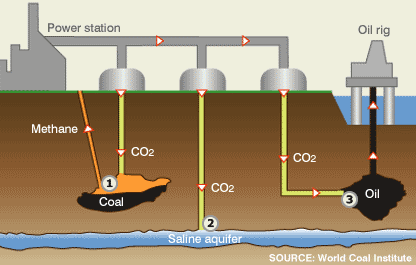
\includegraphics[width=0.5\textwidth]{ccs.png}\label{fig:ccs}
\captionof{figure}{The different ways of CCS} 
\textit{1) CO2 pumped into disused coal fields displaces methane which can be used as fuel 2) CO2 can be pumped into and stored safely in saline aquifers. 3) CO2 pumped into oil fields helps maintain pressure, making extraction easier.}\\

One way to trap the buoyant CO$_2$ is the dissolution of free-phsae CO$_2$ (gaseous state) into the groundwater. This way the CO$_2$ will stay trapped as it is no longer buoyant and this is because as the CO$_2$ is injected the density of water increases so groundwater containing dissolved CO$_2$ will sink toward the bottom of the aquifer. This results in convective flow which sweeps fresh groundwater upward and thereby greatly enhances the rate at which the CO$_2$ dissolves into the groundwater\cite{groundwater}. The understanding of convective dissolution on the lifetime and distribution of a plume of CO$_2$ in the subsurface are very important for risk management. There have been many studies on the issues and great improvements on the understanding of these issues have been conducted. \\
A relevant parametre that comes into play is the Rayleigh number 
$$R = \frac{HK\Delta \rho g}{\text{\O} D \mu}$$
Where $K=d^2/12$ is the effective permeability with d being the gap size between our two glass plates, \O \space is the effective porosity, $\Delta \rho$ is the excess density between CO$_2$-brin and brine, $\mu$ is the viscosity, D diffusivity, g gravity and H the glass plate height.\\ What the Rayleigh number tells us is that it associates the rate of buoyancy driven convection, in our case as the CO$_2$ is being injected from a density increase, with the rate of diffusive transport. We assume constant pressure and rate of CO$_2$ injection (which we do have), in that case the number only depends on the permeability of the medium i.e the ability of a porous material to allow fluids to pass through. Convection will occur if the rate of convection greatly exceeds our system's ability to diffusively distribute the density increase and as we shall see the formation of fingers is the dominant flow pattern in density driven convection flows\cite{Hassan07}.\\
There are many ways to monitor and record the flow process, in our experiment we will be adding BTB in type-2 water that will act as a pH indicator. The main advantage of a colour indicator is for photography as we will be able to directly visualise the patterns and is the easiest way to obtain photographic images of the patterns to analyse. This is also the most widespread technique used and has been used in various other experiments to determine the flow pattern. \\
Bromothymol blue (BTB) is a textile dye derivative that is usually deployed as a pH indicator whose protonated and deprotonated forms makes it a very good indicator of dissolved CO$_2$. We will not go into much detail into the theory of BTB as experiments have shown it has little on the mechanisms of the patterns that are being formed\cite{BTB}.

\section{Methods}
\subsection{Material}
The main components for our experiment will consist of two glass plates glued together with a gap between them. We have in the following conducted our experiment with two different sets with different dimensions. The first set\\

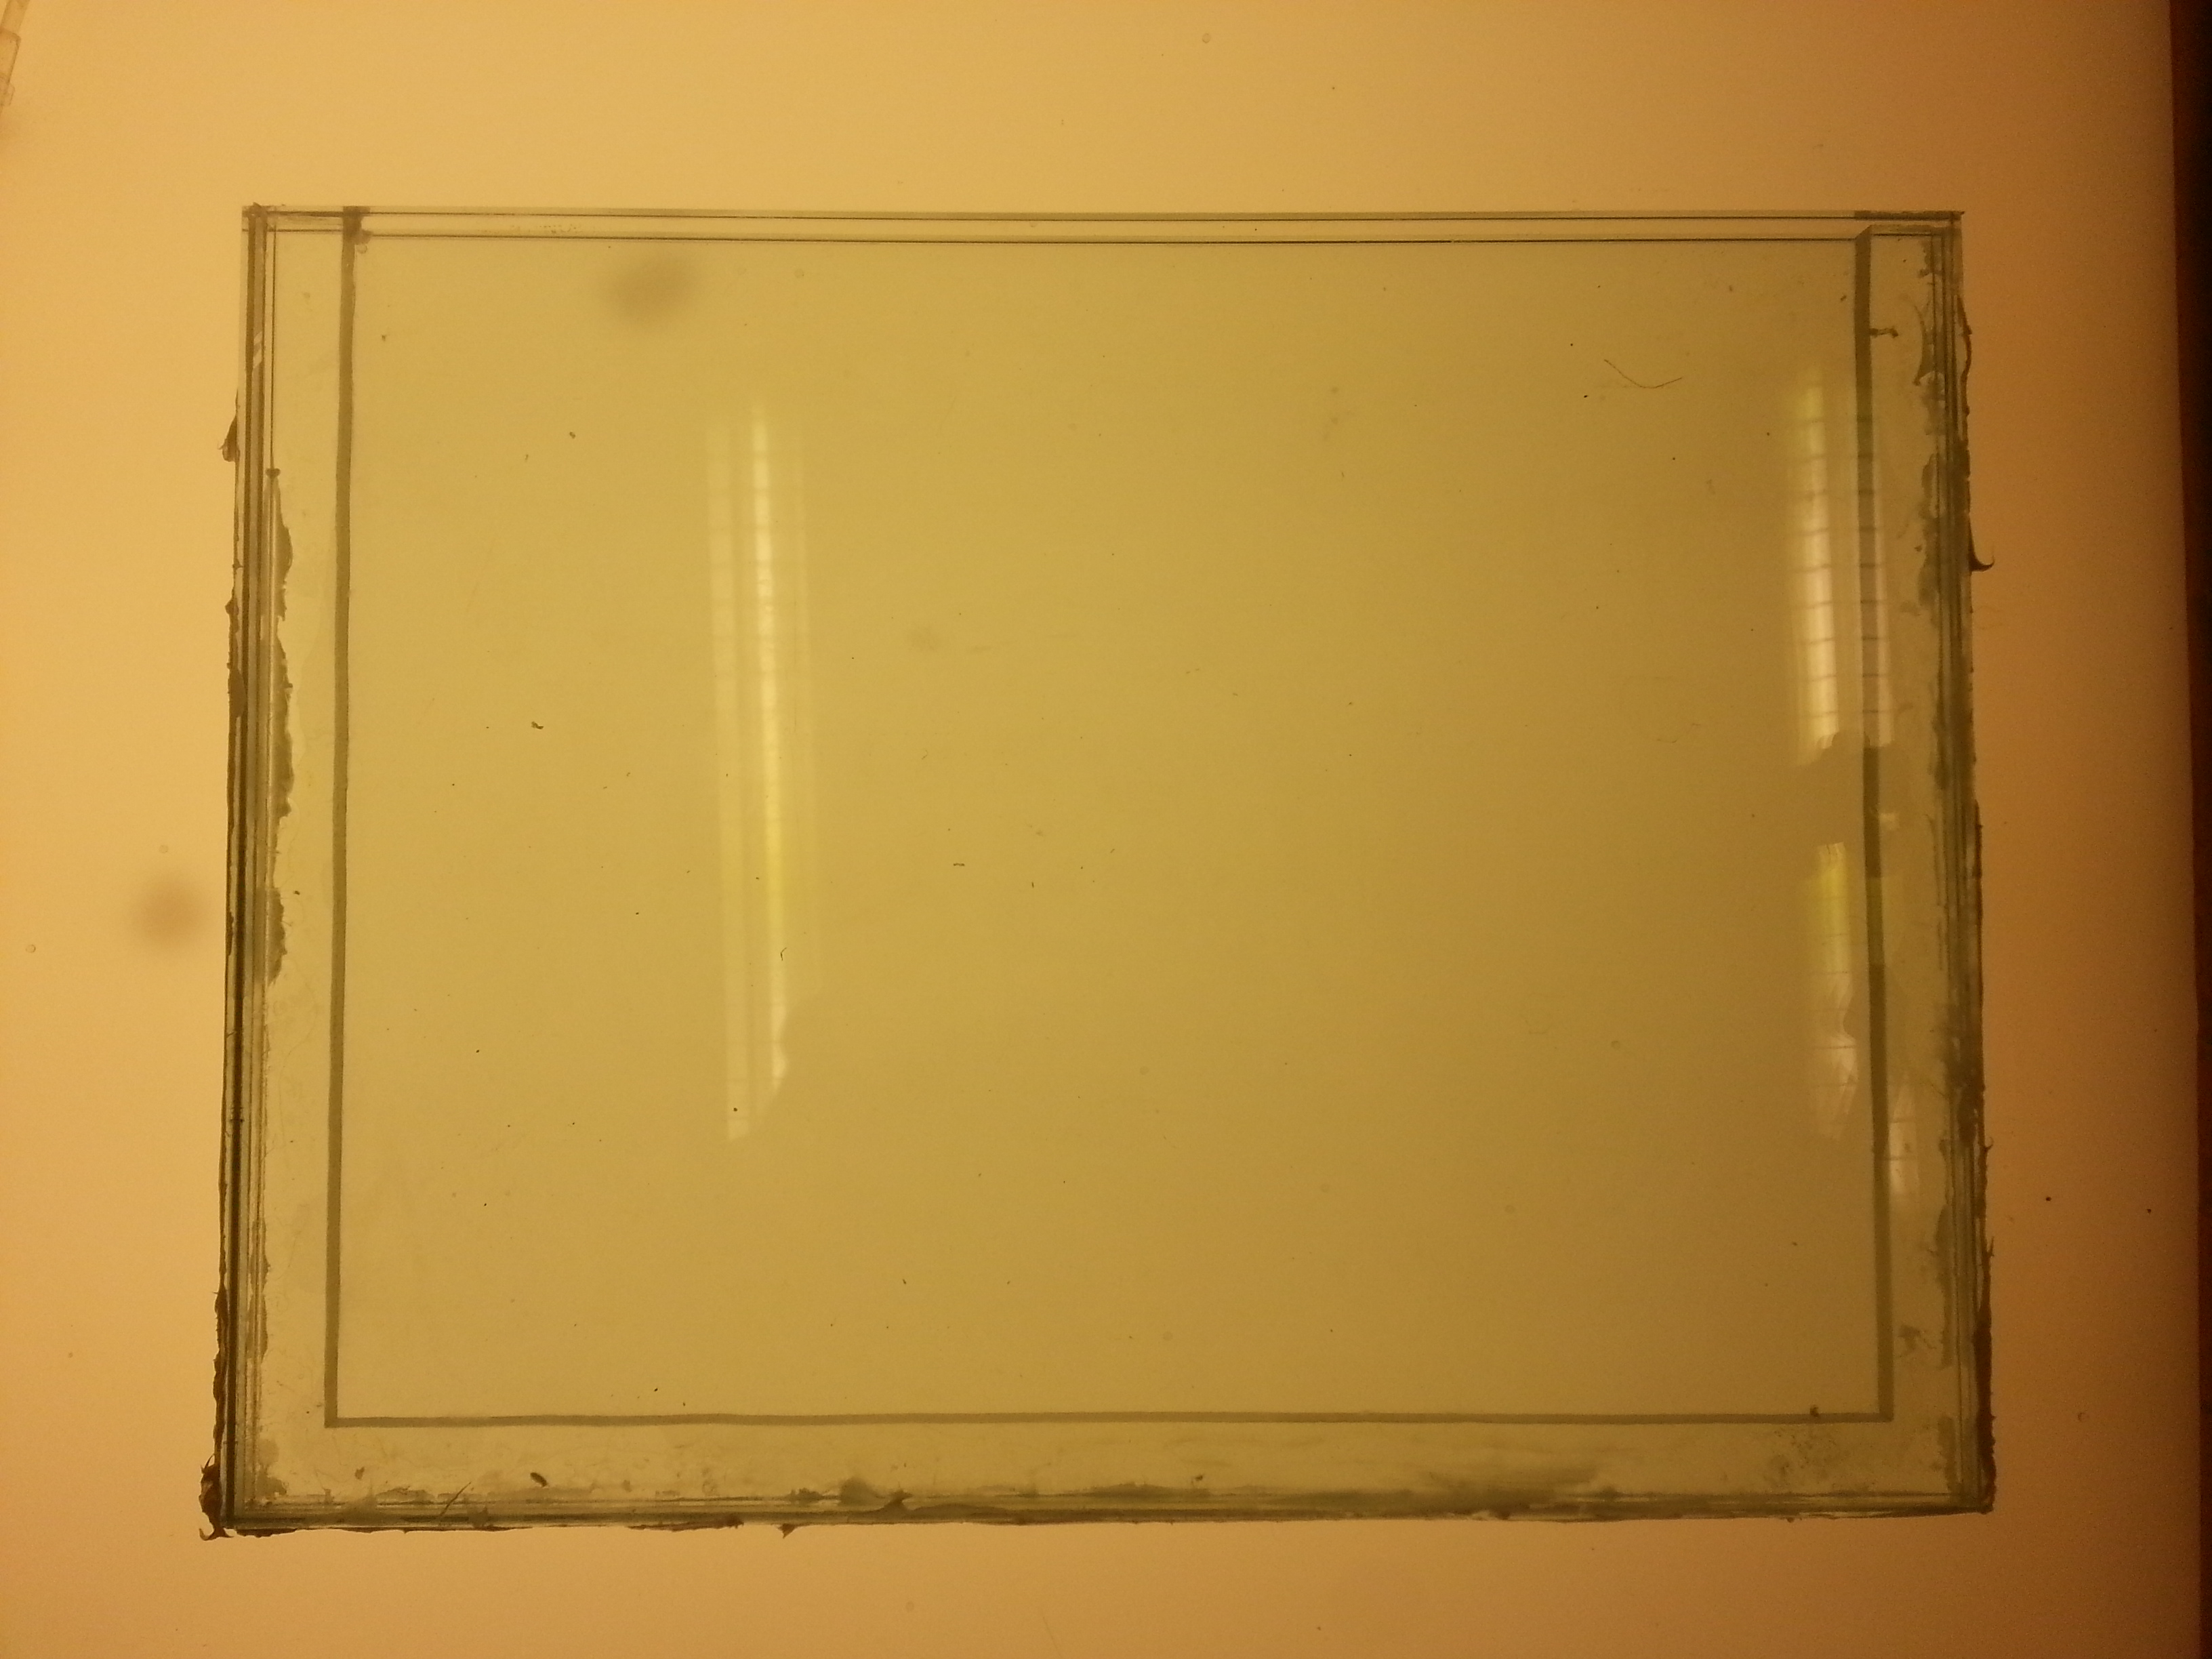
\includegraphics[width=0.42\textwidth]{plate1.jpg}\label{fig:plate1}
\captionof{figure}{Our initial plate} 
\vspace{0.2cm}
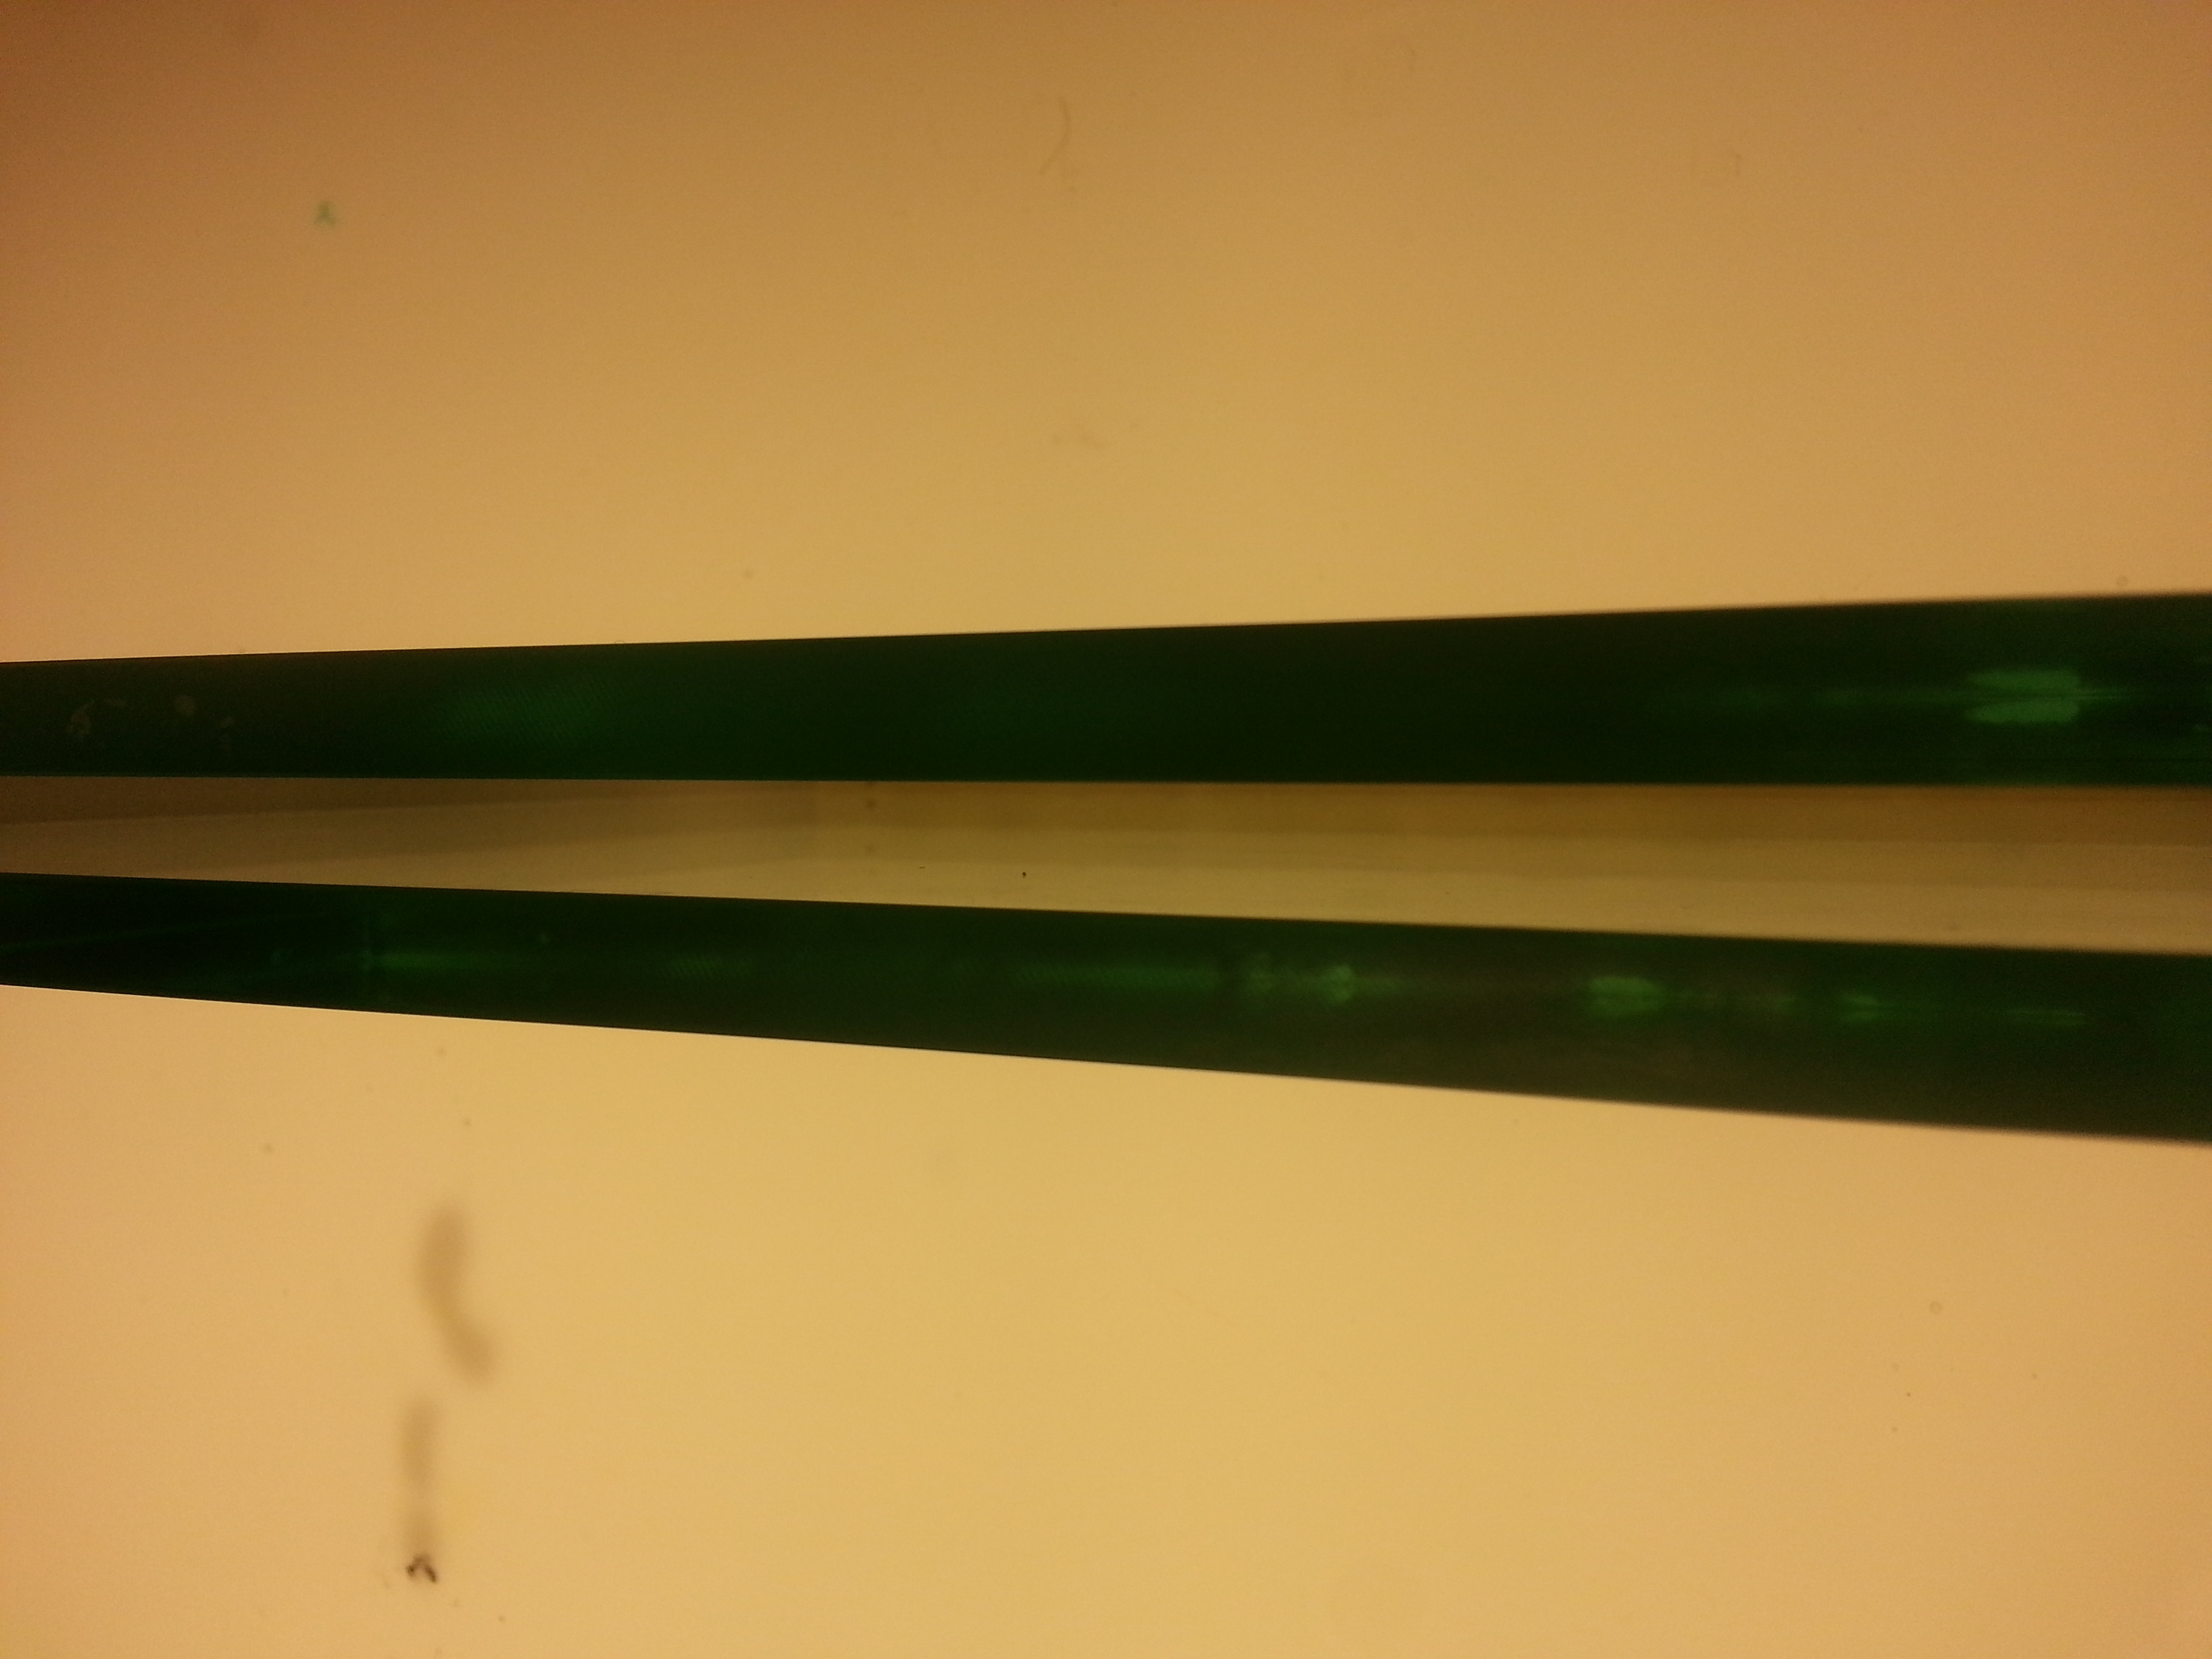
\includegraphics[width=0.36\textwidth]{plate1g.jpg}\label{fig:plate1g}
\captionof{figure}{The gap in which our solution and beads went into}

had the dimension of approximately $40\times 37$cm in length and height, the depth of the glass plate set up was $2.7$cm and the gap as shown in the second image was $0.9$cm. We had the vertical sides and the bottom sealed with super glue and silicon glue to make it leakage proof. \\ 
Our second set up \\

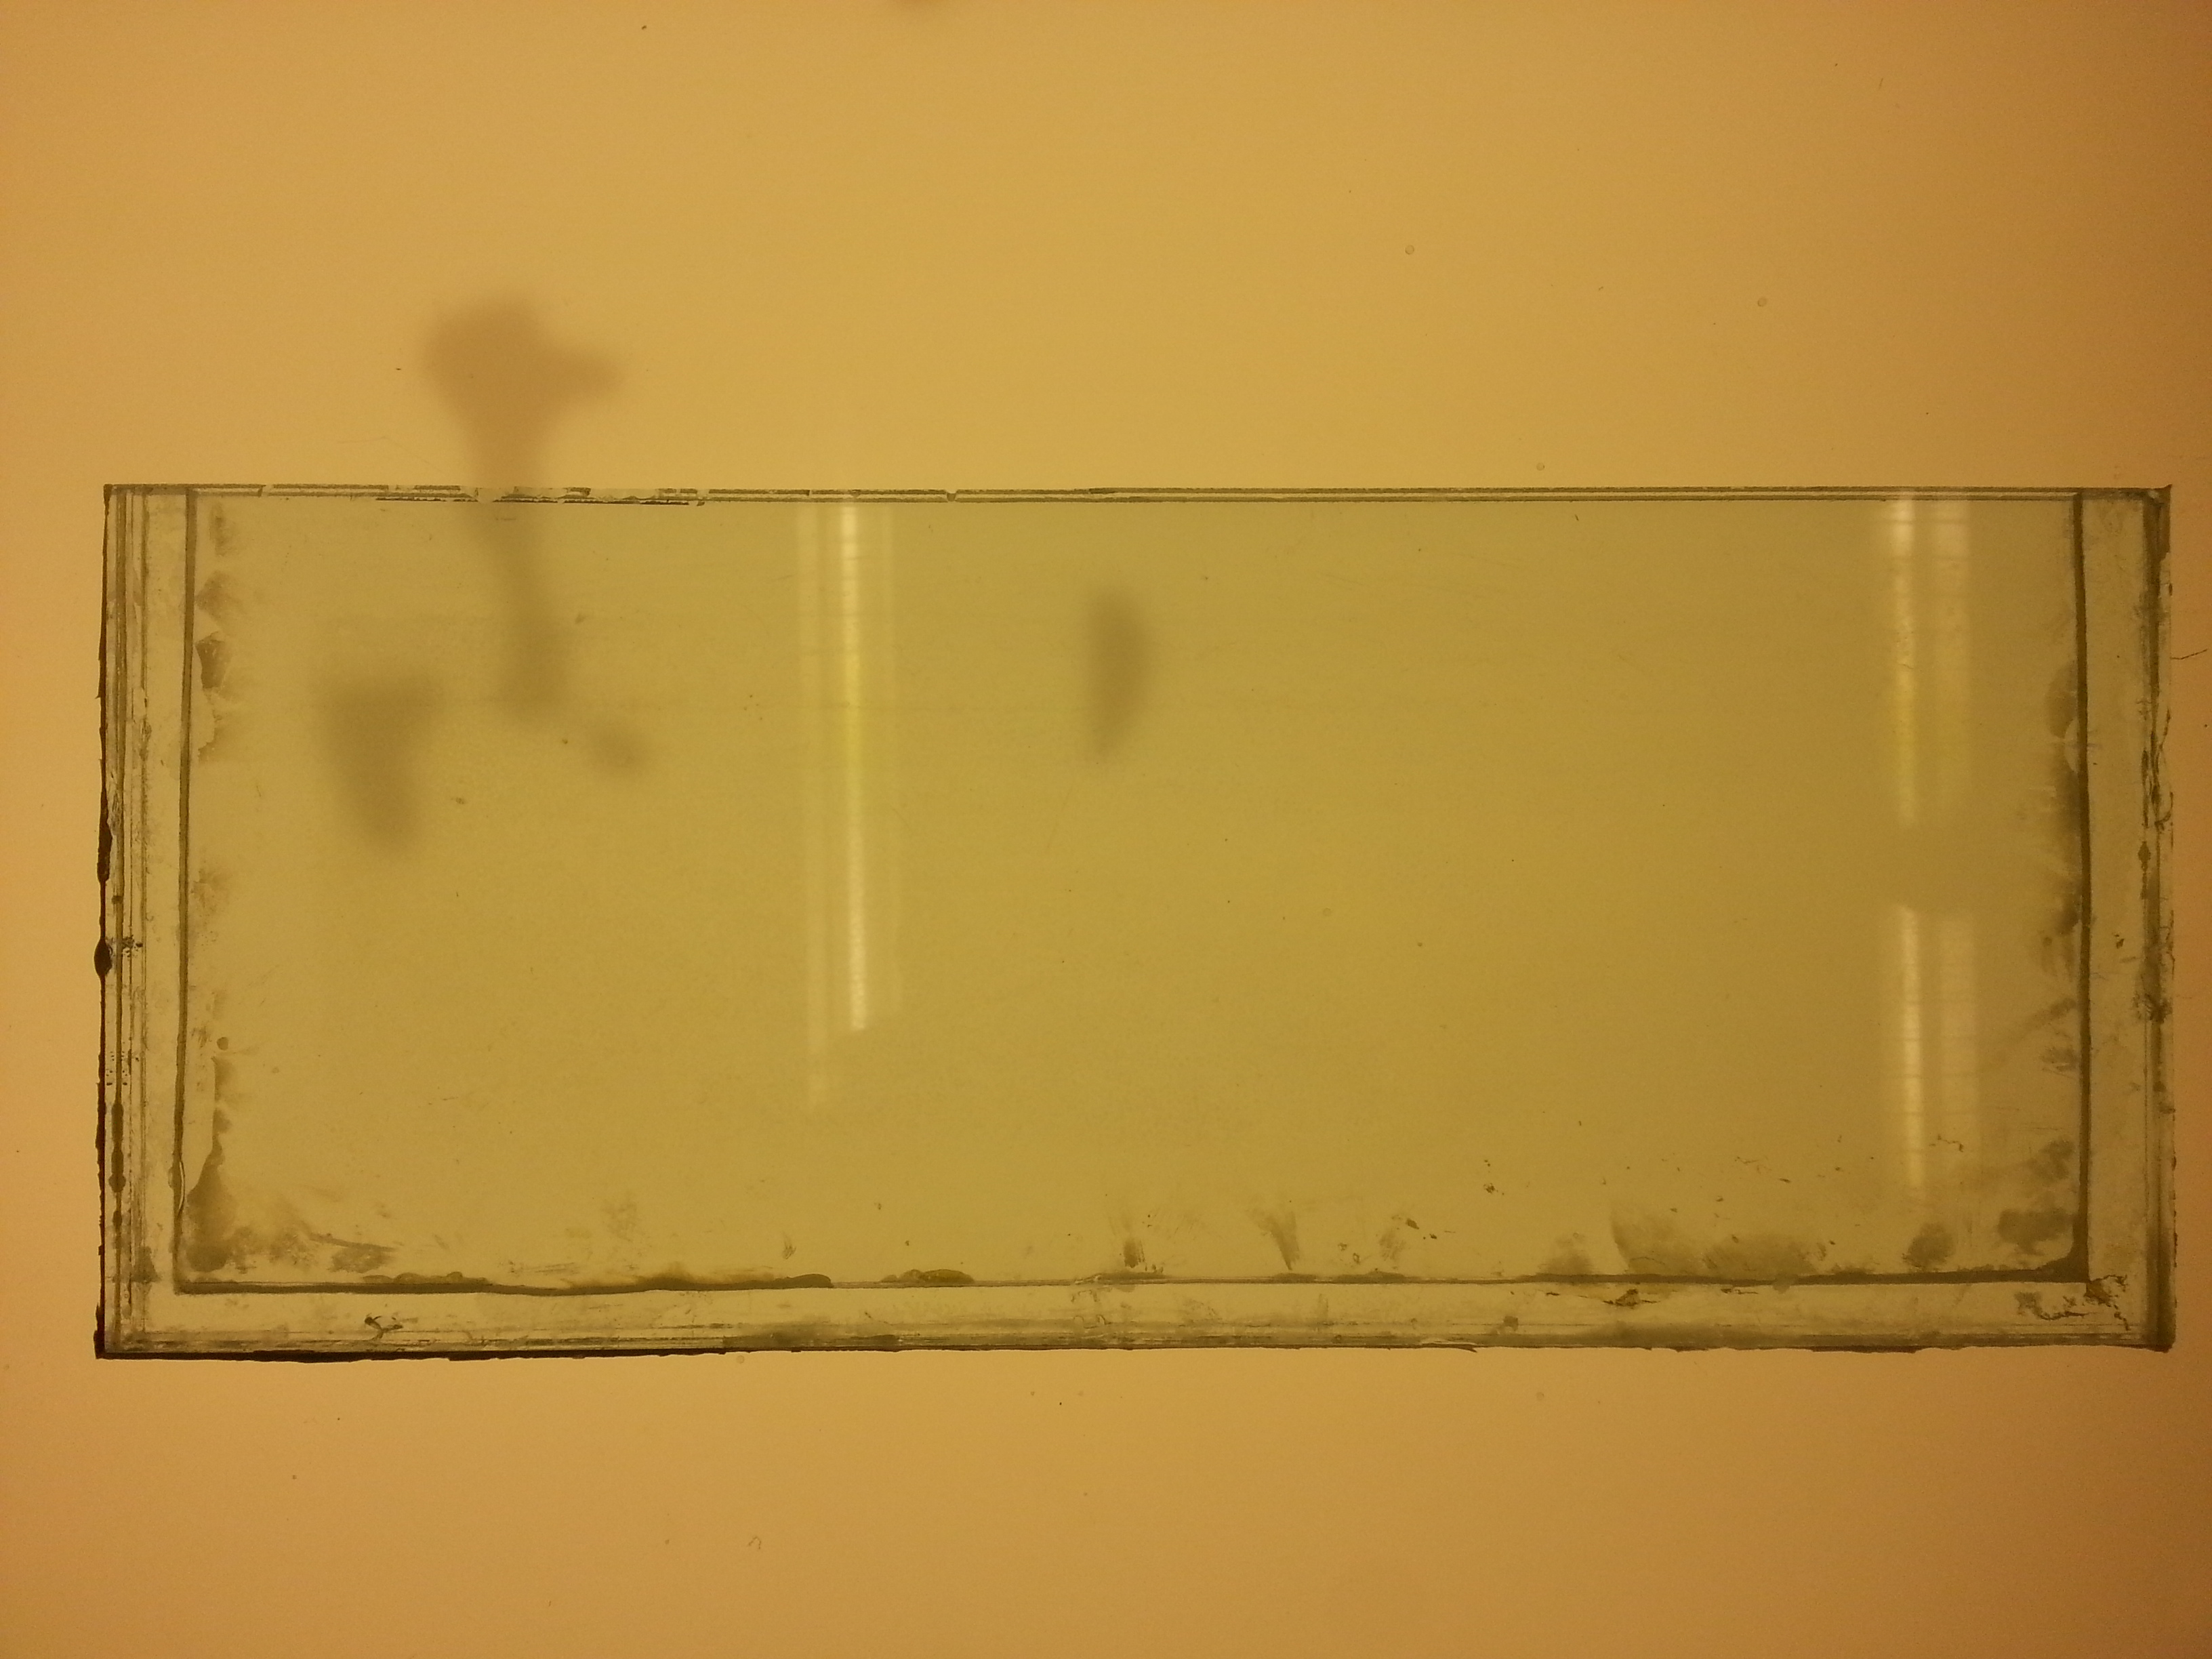
\includegraphics[width=0.42\textwidth]{plate2.jpg}\label{fig:plate2}
\captionof{figure}{Second glass plates which was thinner but longer}
\vspace{0.2cm}
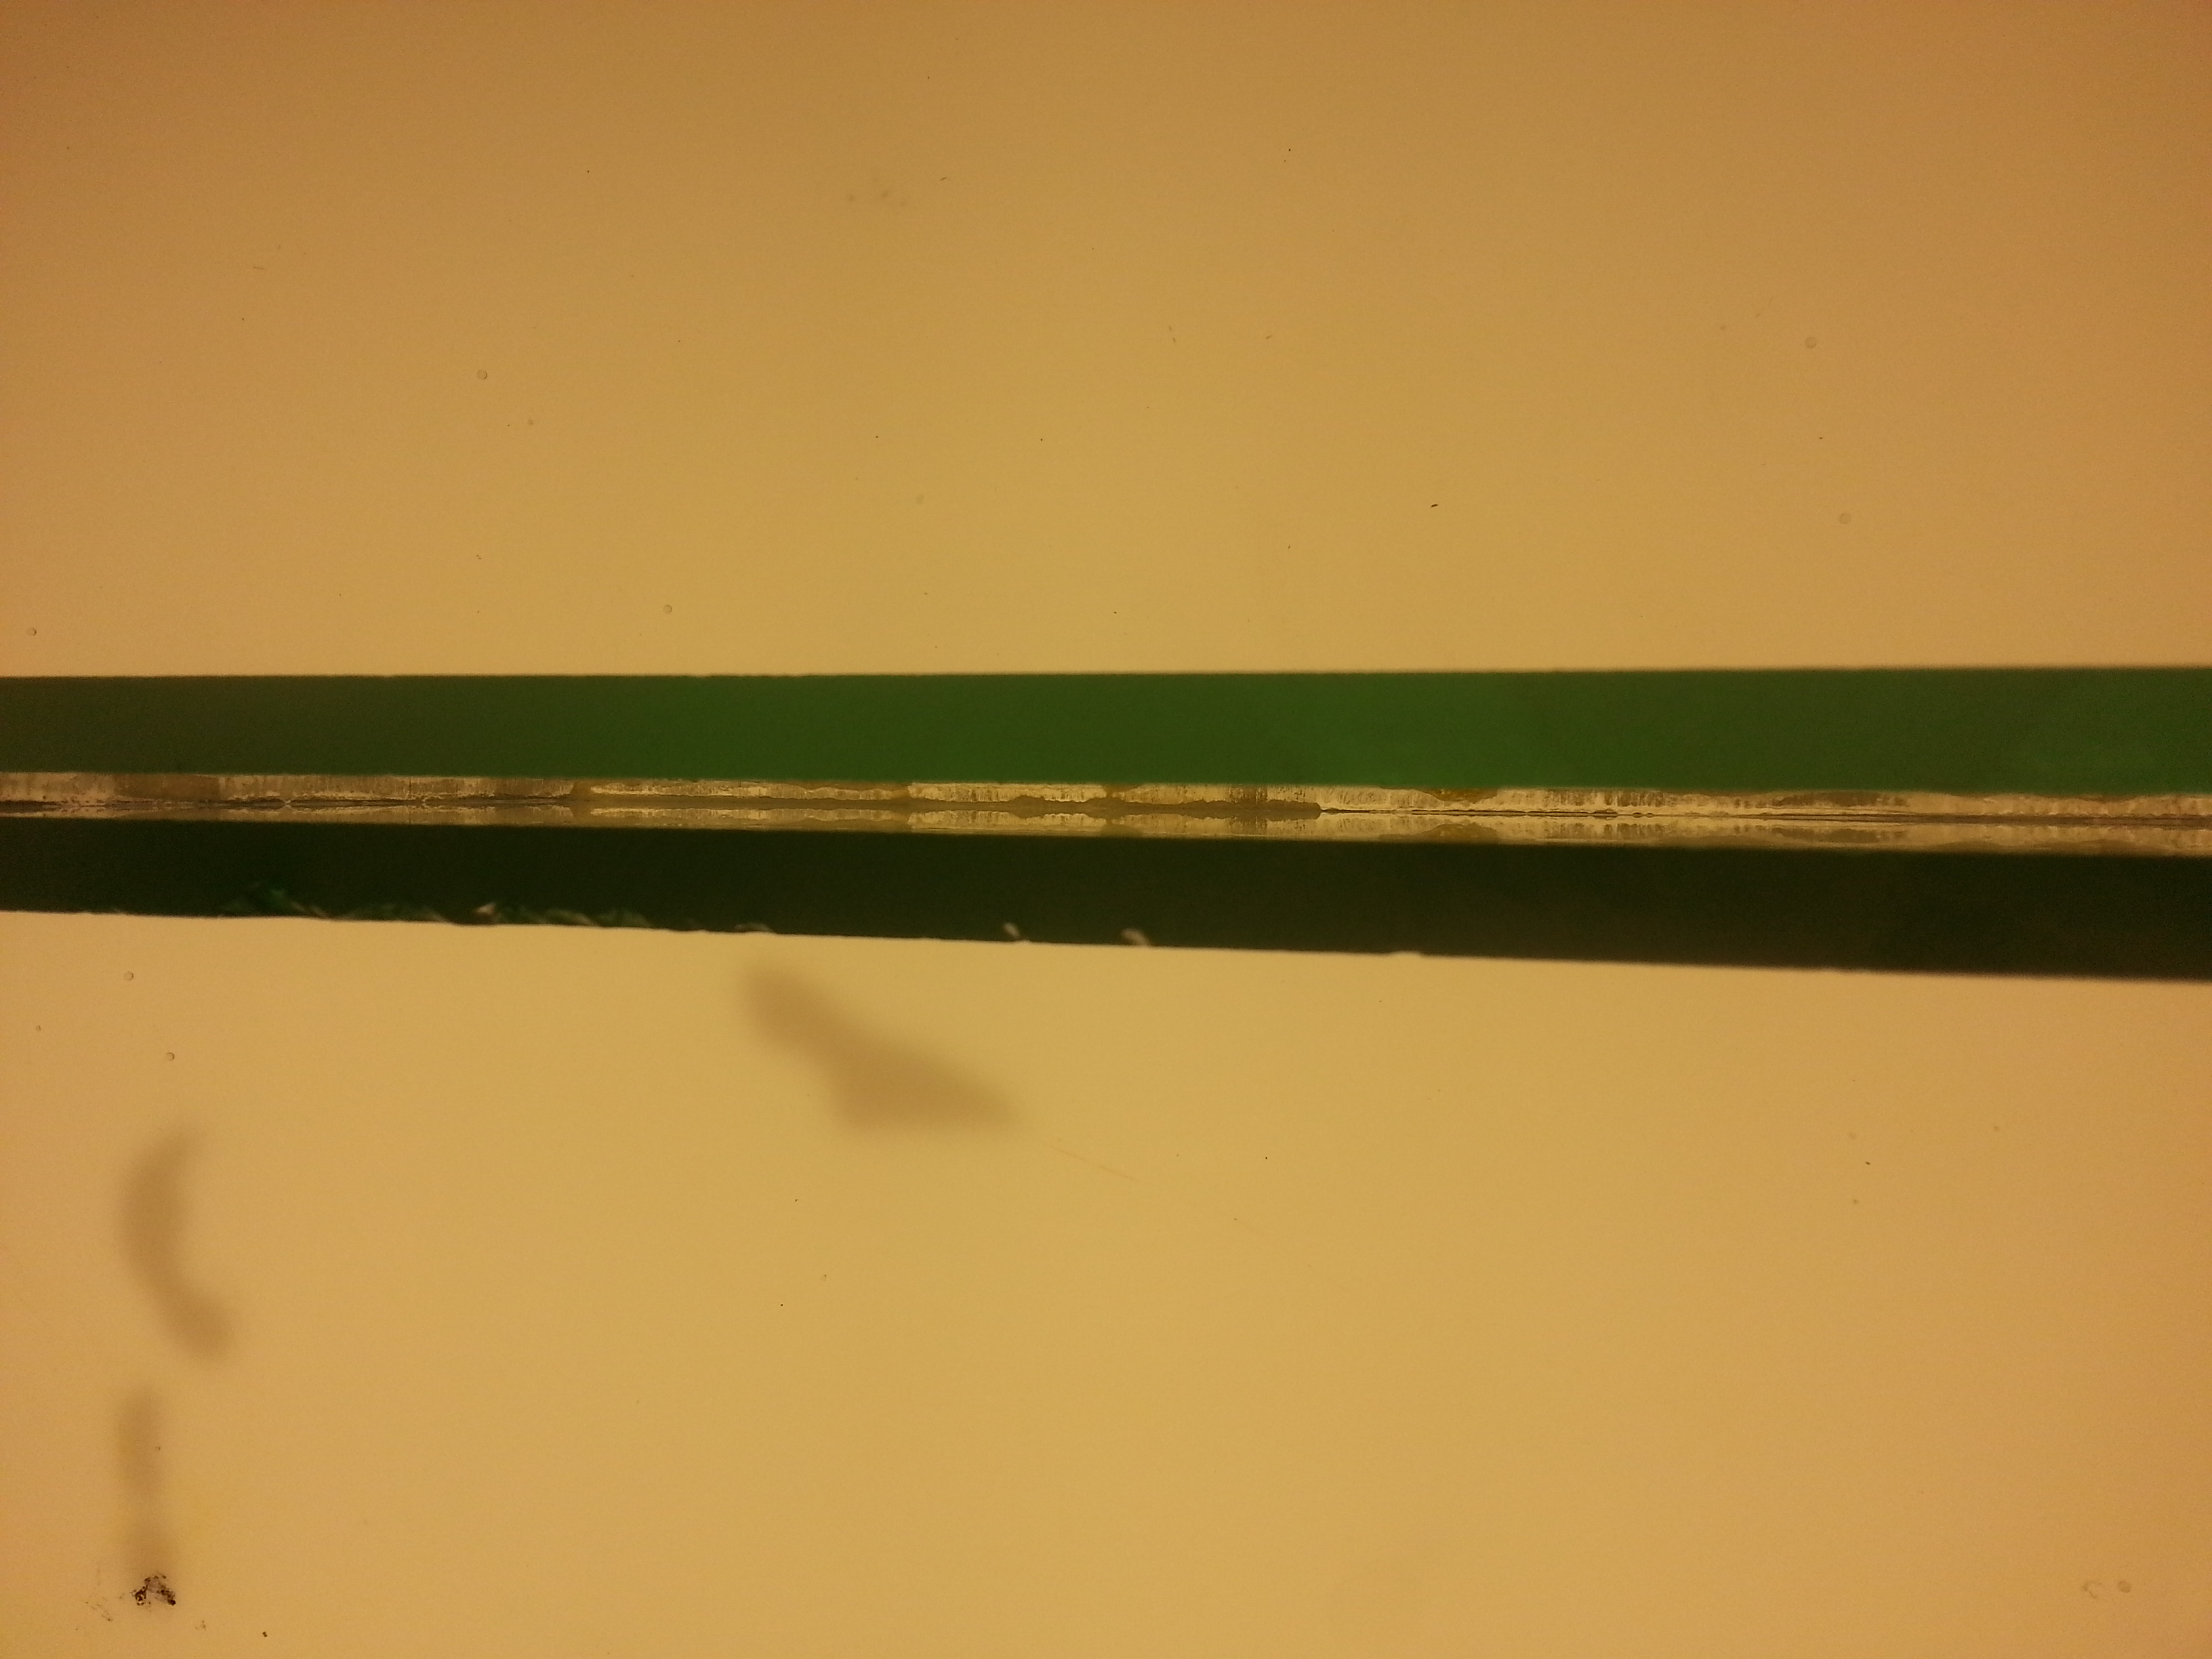
\includegraphics[width=0.38\textwidth]{plate2g.jpg}\label{fig:plate2g}
\captionof{figure}{The gap which as seen is narrower than our previous set up}
\vspace{0.3cm}
had the dimensions $50 \times 27$cm in length and height with $2.5$cm as the depth and the gap measured at $0.5$cm. We had as previous the bottom and the vertical sides glued with super glue, but no silicon glue this time as it proved to be not of vital significance last time.\\
We used type-2 water which is purified water used in laboratories with no excessive traces of minerals or other chemical elements that could potentially affect our experiment. Our initial BTB solution was $0.2$g/L, but this amount changed as the experiment progressed.\\
During our experiments we used glass beads with various sizes ranging from $3$mm - $1$mm\\
For recording and monitoring our experiment we used a DSLR (Digital Single Lens Reflex) camera body with a lens. For the camera to capture the patterns as they are forming during the injection vividly. 

\subsection{Set up}
We had a large approximately $1.5 \times 1.5$m lightbox leaning against the wall while we had our system set up on a table with the camera in front. \\

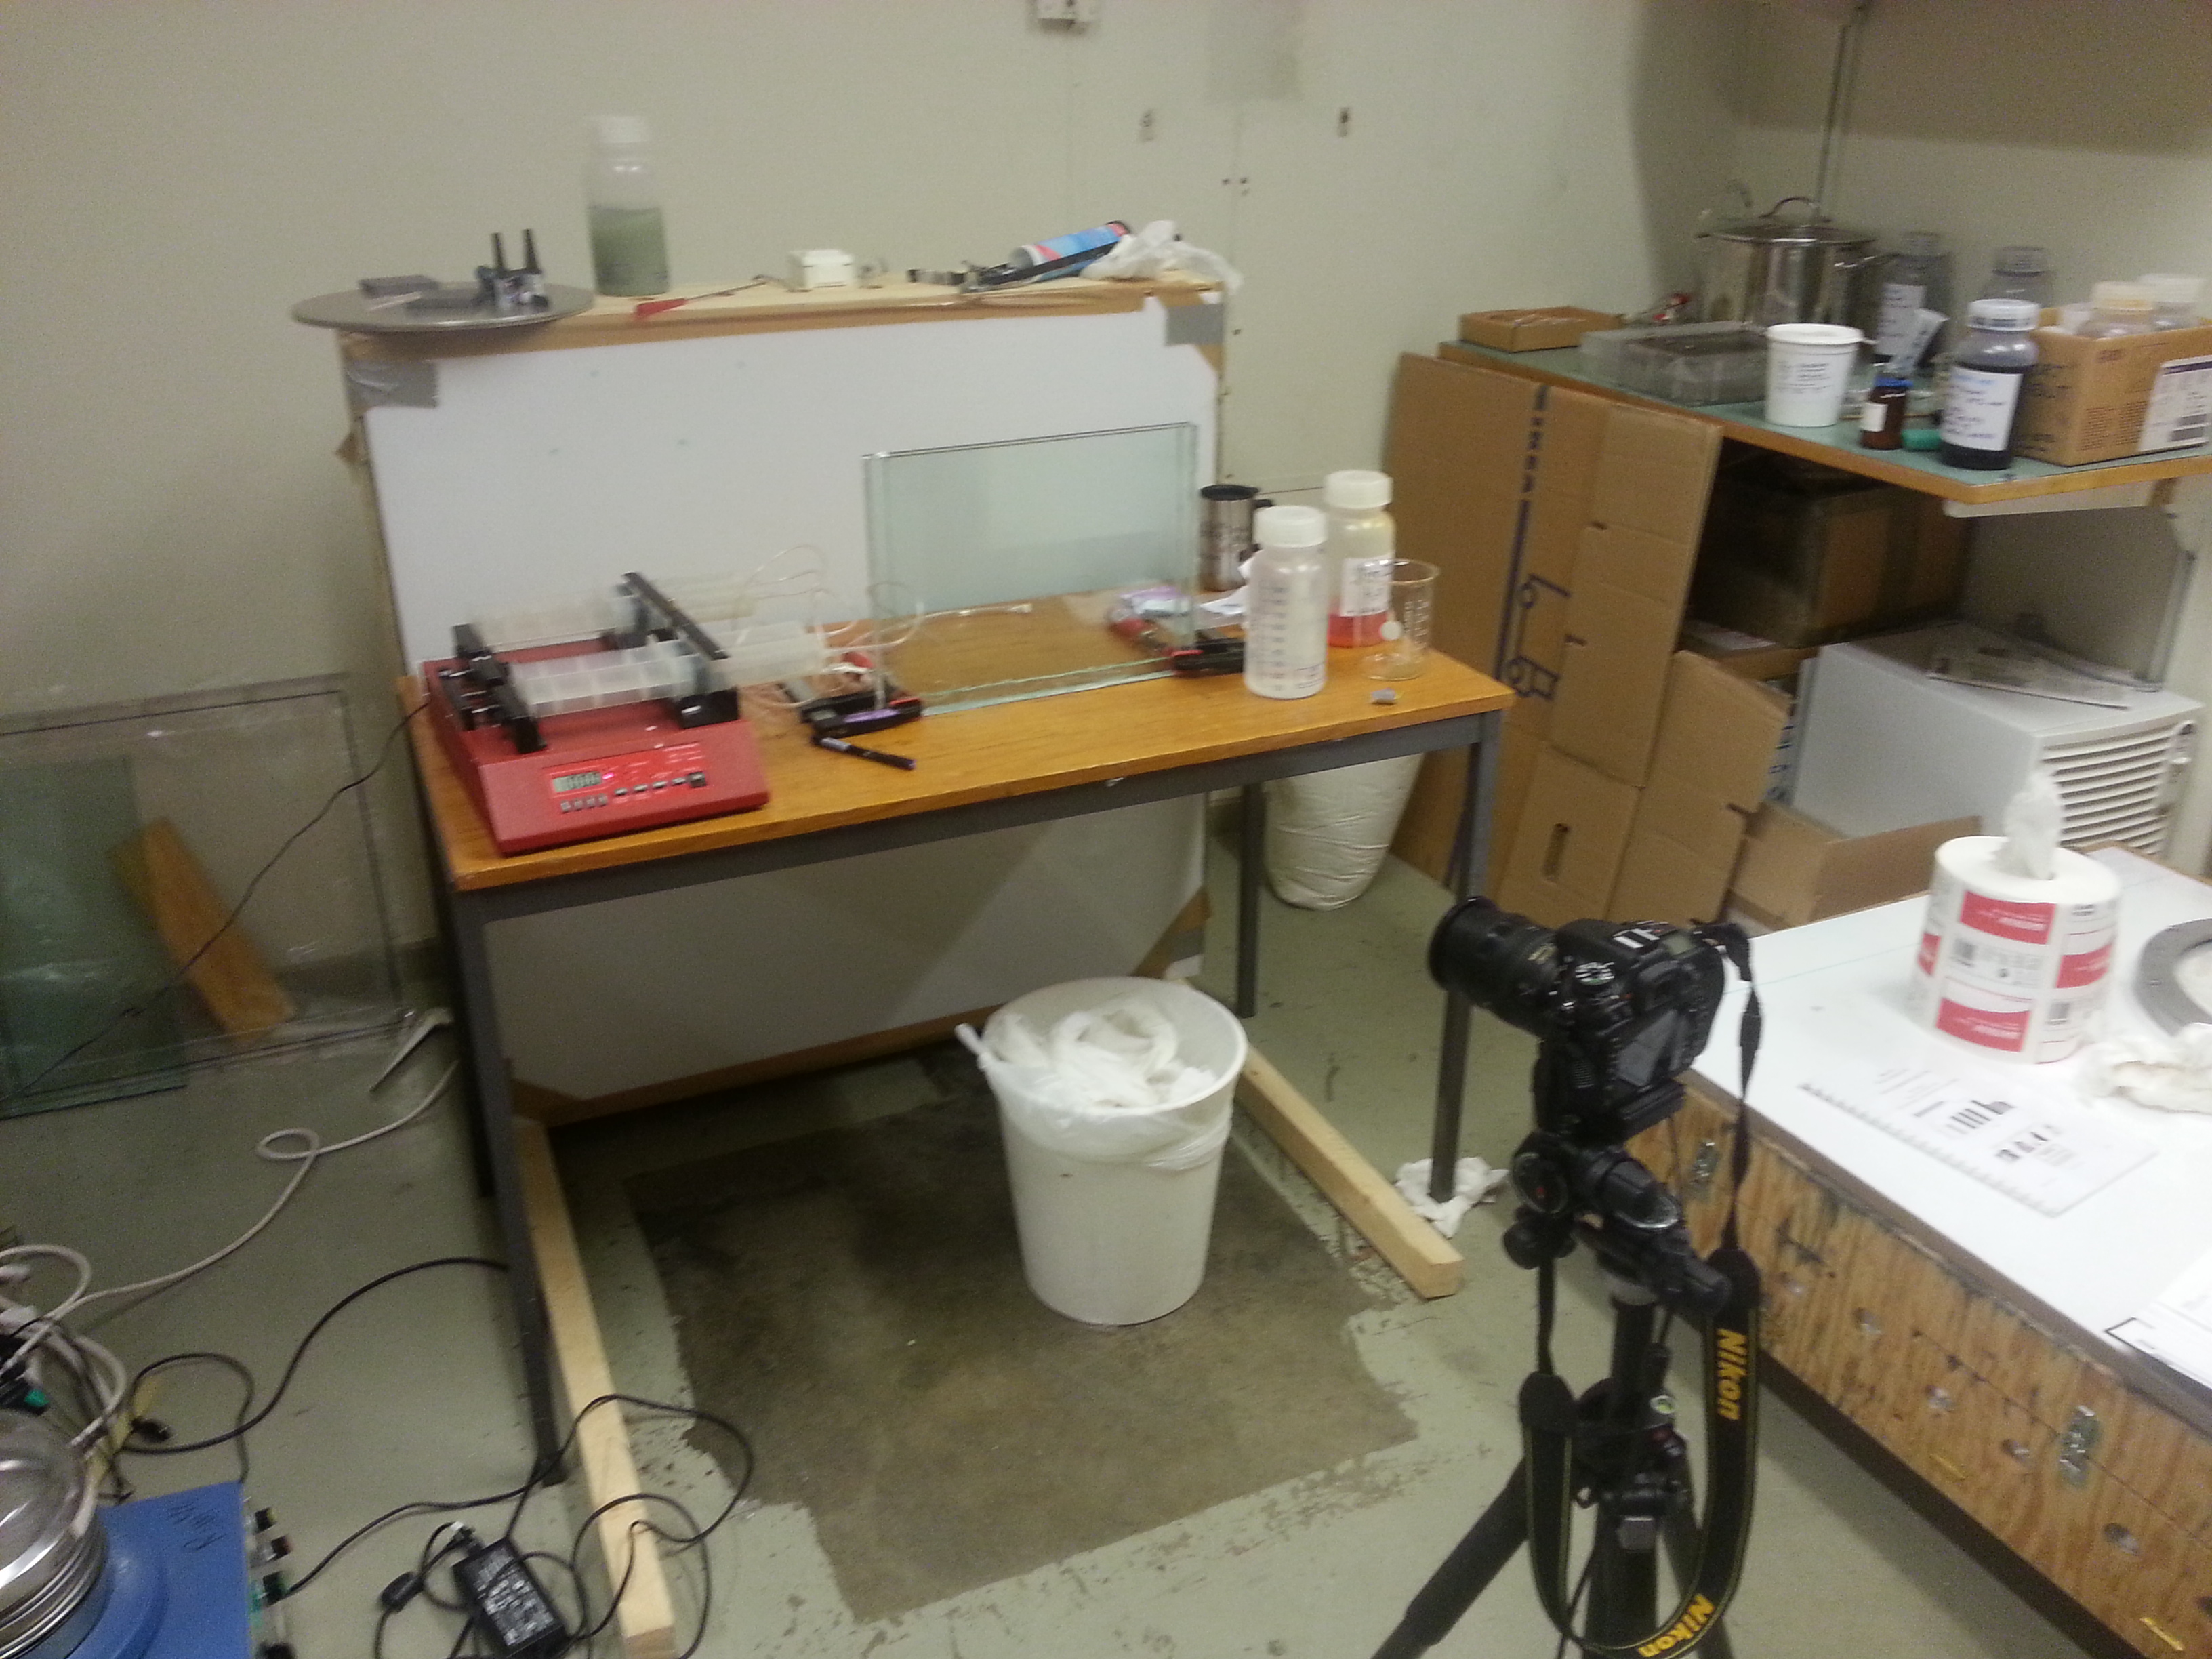
\includegraphics[width=0.45\textwidth]{setup.jpg}\label{fig:setup}
\captionof{figure}{Our initial set up of the experiment}
\vspace{0.3cm}
The camera seen above is a NIKON D7100 with a focal length $40.0$mm, ISO speed rating of $100$ and exposure time $1/30$sec. As previously mentioned we used intervals of $5$min between each image taken by the camera. As the camera was recording the process with an interval of $5$min, we had a pump set up to inject CO$_2$ into our system at a rate of $10$ml per hour with a maximum limit set to $100$ml. The pump system \\

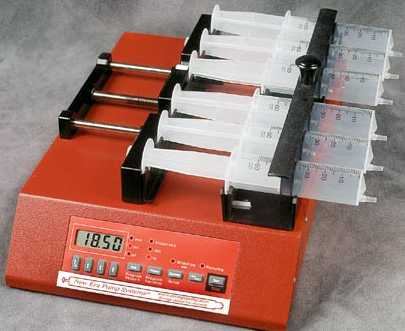
\includegraphics[width=0.34\textwidth]{pump.jpg}\label{fig:pump}
\captionof{figure}{The programmable syringe pump system}

we used is shown above, but as opposed to the image we only used four channels i.e we had four syringes filled with gaseous CO$_2$. This type of pump allows one to adjust the flow rate and maximum rate among other functions that can be adjusted. \\
The lightbox mentioned consisted of several fluorescent lamps illuminating the background of our system so the camera could capture the moments. \\
We shifted to a led variant further in the experiment which would emit less heat, but this is of no concern as those in the experimental group of last year have tested out the effect of heat from the lightboxes are of minimal concern.\\ 
On the other hand what does affect is the colour of our lightsource, we would want our lightsource colour to be on the colder side of the scale. This is of importance later on during the image processing.\\
Furthermore each syringe had a tube connected to it and all the tubes would then get connected to a master tube that would be places on the top of our system between the gap. We initially had $500$ml of our BTB solution poured into our system using our initial plate and then filled it with glass beads. For our initial experiment we used glass beads of $1$mm size using our initial plate. The master tube would then cover the top of our system and fill the gap, the tube had a hole around the middle so the CO$_2$ could diffuse into our solution. \\ 
After each experiment we would refill the syringes with new CO$_2$ and pour the wet beads onto a plate to dry. We could either use the oven to dry the beads or just leave them overnight spread over the plate in as thin layer as possible for them to dry. We would then wash the glass plate inside and out with tap water and dry it with a pump. This was just a precaution so that no external sources would affect our new experimental set up (such as some leftover solution from previous experiment or green coloured beads). All experiments were conducted under room temperature and pressure conditions.\\

\subsection{Analysis procedures} \label{analysis}
For the analysis we turned to FIJI ImageJ\cite{imagej} which is an image processing software designed for scientific use ranging across many disciplines. In our processing we used the Linux version as we were working on a Linux system, but the OS X and Windows versions should be alike, we assume here no difference between them. The software is Java-based and once compiled to fit your system should be relatively fast at handling the vast data captured by camera. This is a very powerful software which is hard to master, so we will here go step by step explaining how we did it.\\

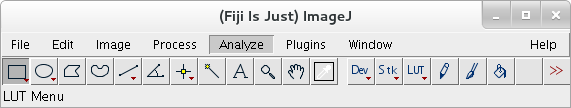
\includegraphics[width=0.5\textwidth]{imagej.png}\label{fig:imagej}
\captionof{figure}{Main window of ImageJ}
\vspace{0.3cm}
We load all photos by going into \textit{File}$\longrightarrow$ \textit{Import} $\longrightarrow$ \textit{Image Sequence...}
Once all the photos are loaded (this might take a while depending on the computation power of your system and whether you have optimised ImageJ for your system), we can go on setting up the conditions for analysing them. What we would like to calculate is the area of the fingers as they evolve over time (in our case every $5$min).\\ 
Once all images are loaded, we load the first image of the stack by \textit{File} $\longrightarrow$ \textit{Open}. At this point one might want to scale the images so as they do not consume too much computer power (if the image files are too big e.g 6000x4000), a scaling of $20\%$ will do. Once we have done that we can go to \textit{Analyze} $\longrightarrow$ \textit{Image Calculator...} we will then have the stack we first loaded as \textit{Image1} and the single image we loaded as \textit{Image2} and then have the \text{Operation} as \textit{Difference}\\

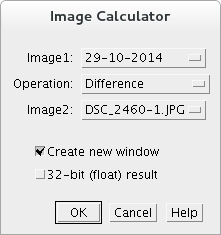
\includegraphics[width=0.45\textwidth]{diffmenu.png}\label{fig:diffmenu}
\captionof{figure}{Sample on how the difference should be taken (v1.49j10)}
\vspace{0.3cm}
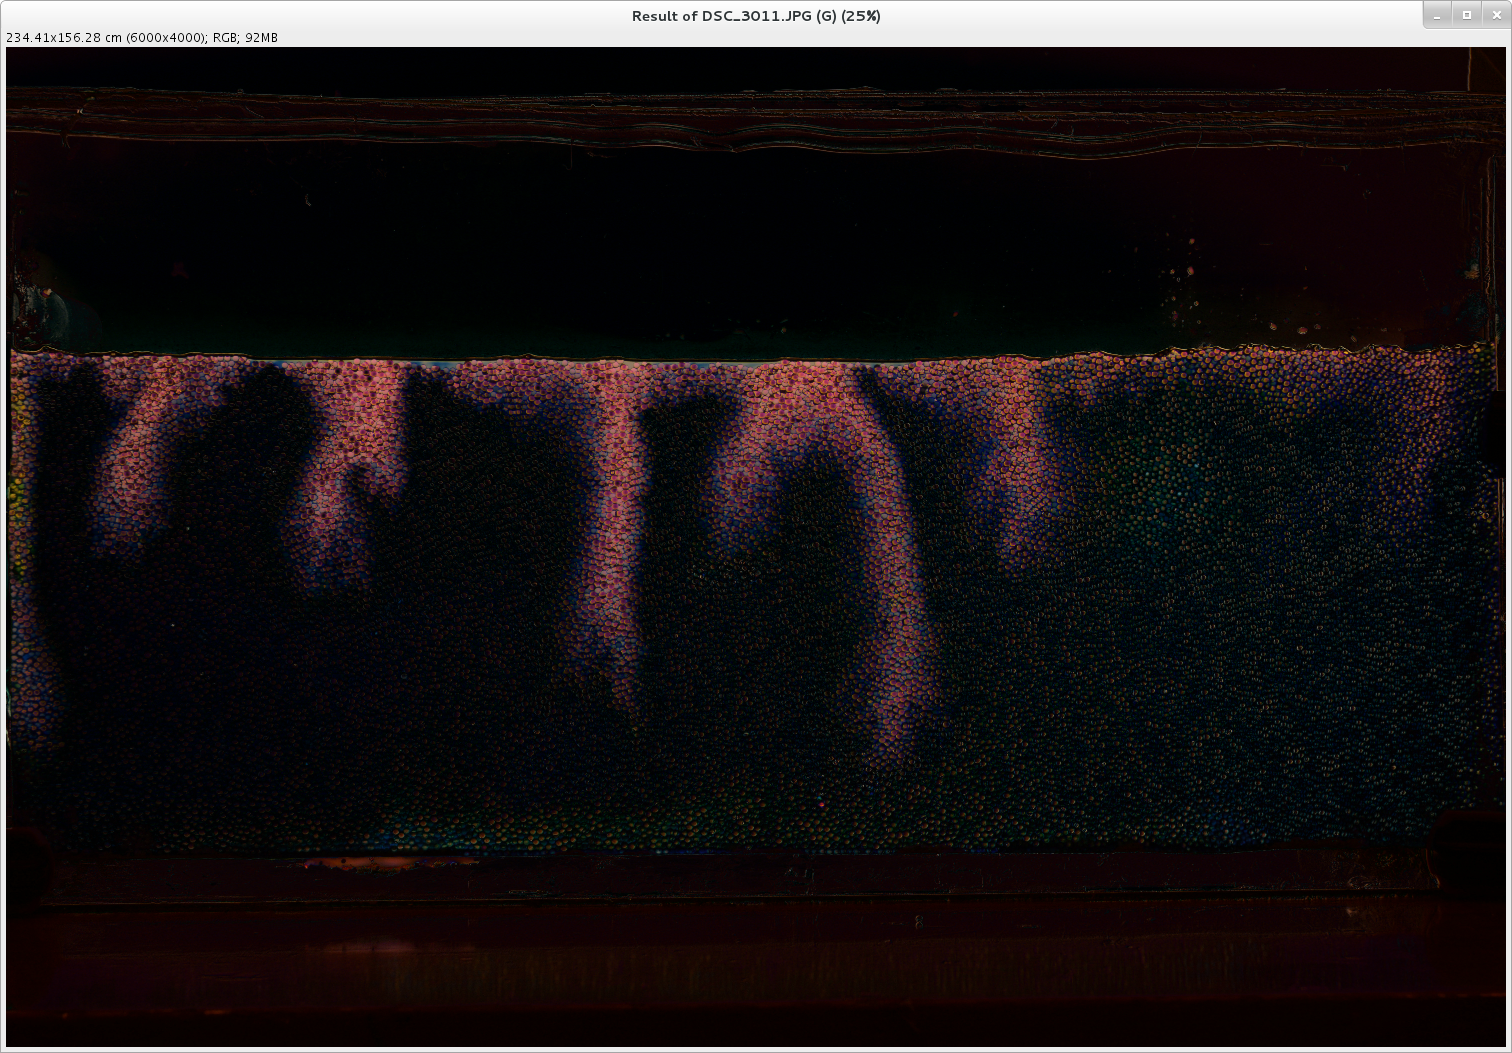
\includegraphics[width=0.5\textwidth]{diff.png}\label{fig:diff}
\captionof{figure}{Sample of the difference}
\vspace{0.3cm}

Next thing we want to do is covert the new image we have gotten on our screen with the difference taken and convert it to $8$bit this can be done by: \textit{Image} $\longrightarrow$ \textit{Type} $\longrightarrow$ $8$ bit. \\

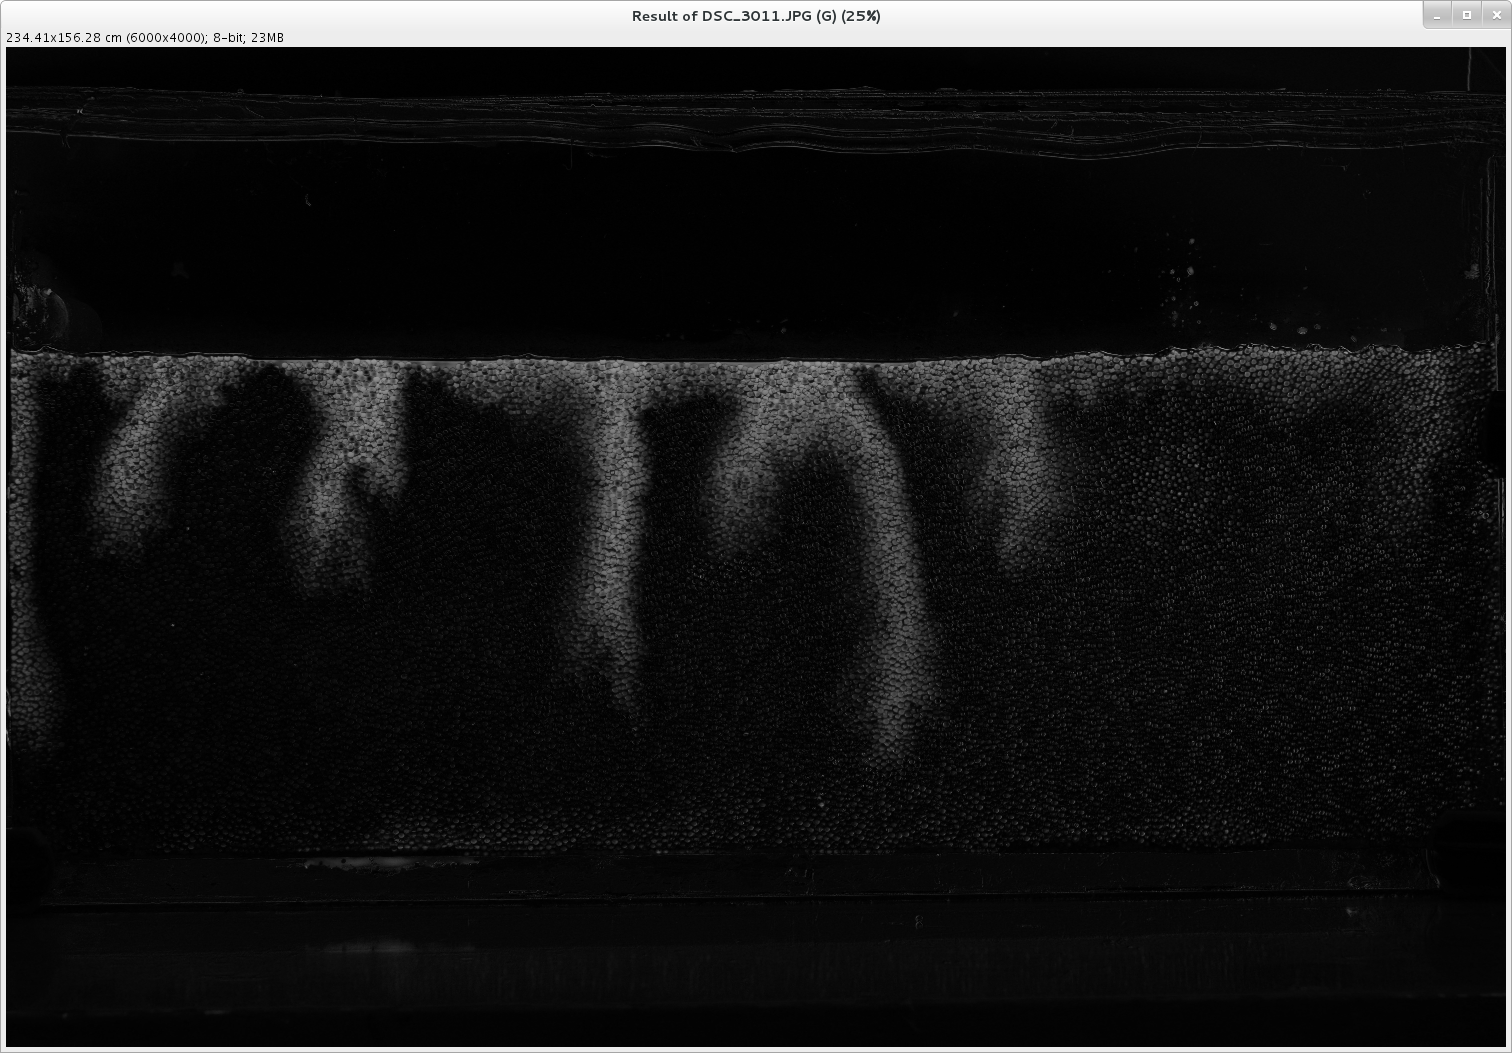
\includegraphics[width=0.5\textwidth]{bit.png}\label{fig:bit}
\captionof{figure}{Sample of an image after converting it to 8bit}
\vspace{0.3cm}
Once this is done we take adjust the threshold by \textit{Image} $\longrightarrow$ \textit{Adjust} $\longrightarrow$ \textit{Threshold} here comes the tricky part, we want to adjust it such that the fingers are in contrast with everything else (there will be some noise, it is inevitable). This is also why the lightsource colour is important as previously mentioned, if the lightsource emits warm colour then adjusting the threshold will be harder, from what we have experienced.\\ 

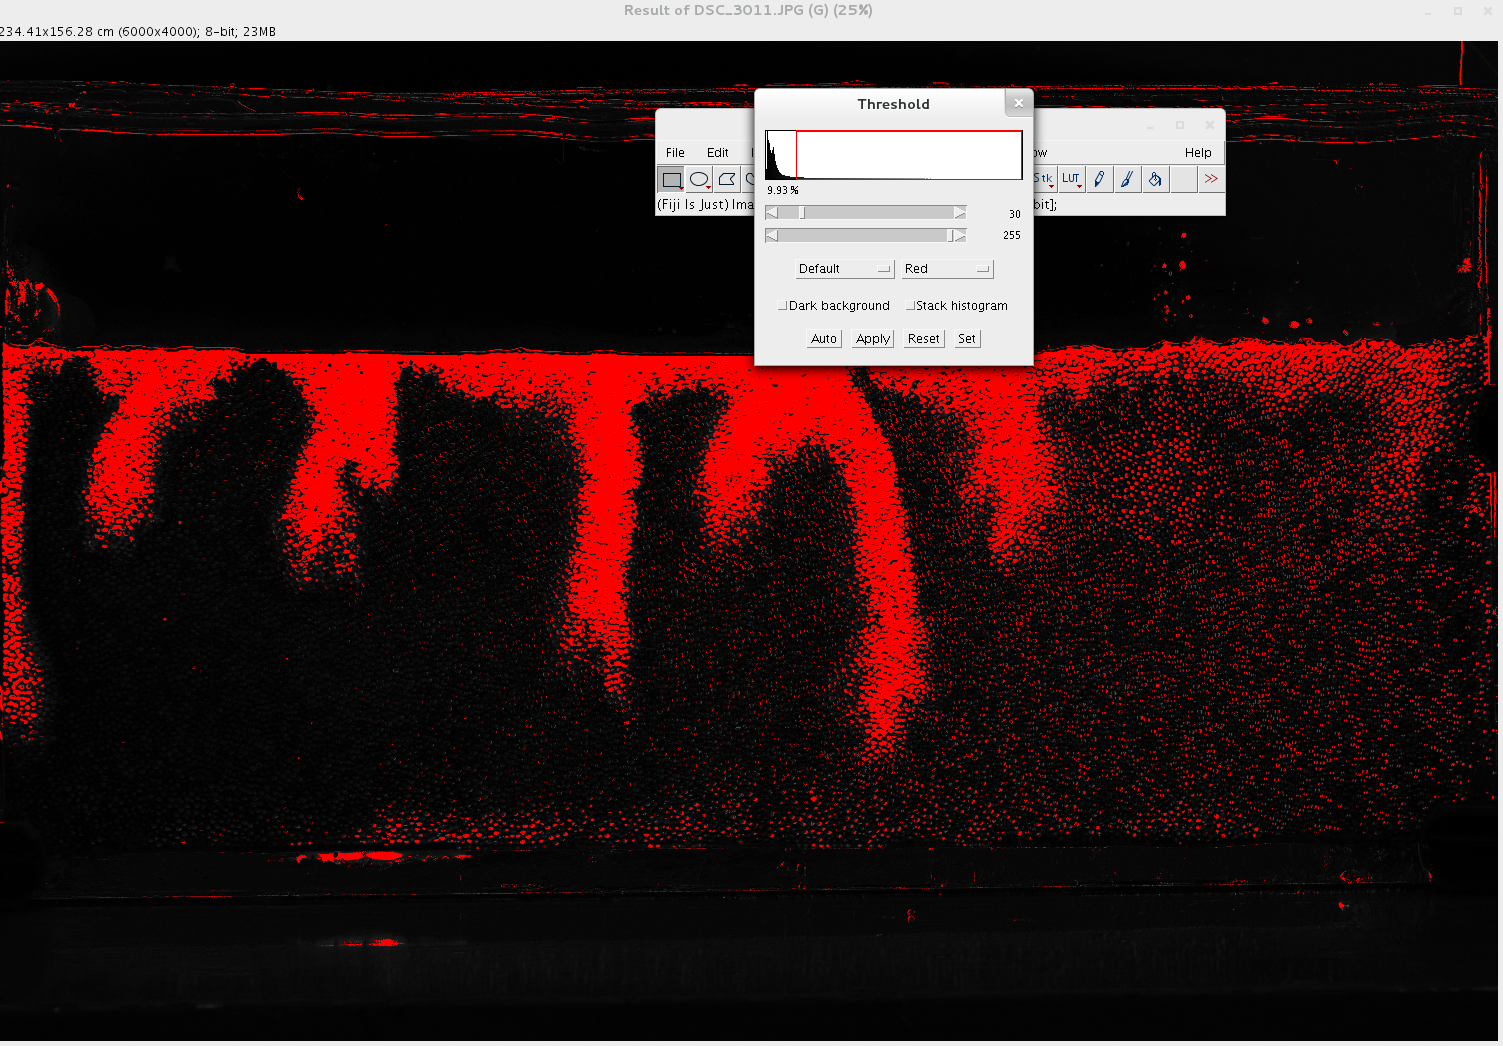
\includegraphics[width=0.5\textwidth]{thresh.png}\label{fig:thresh}
\captionof{figure}{Sample of threshold}
\vspace{0.3cm}
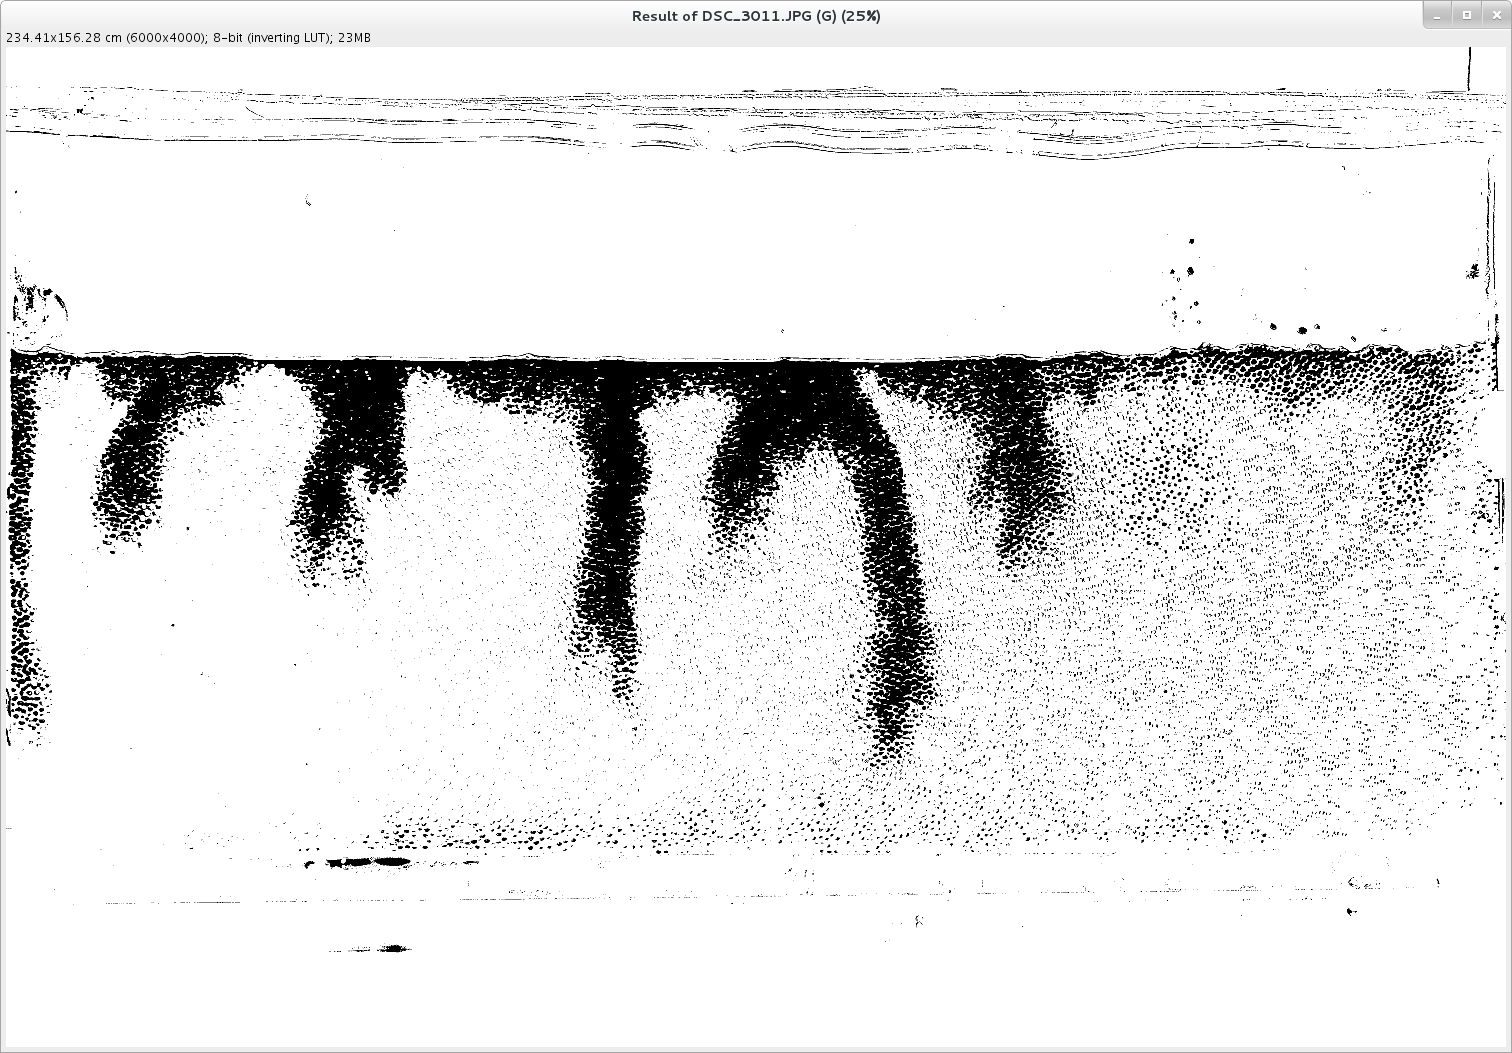
\includegraphics[width=0.5\textwidth]{final.png}\label{fig:final}
\captionof{figure}{Sample after taking the threshold}
\vspace{0.3cm}
If there is a considerable amount of noise one could try to reduce them by \textit{Process} $\longrightarrow$ \textit{Noise} $\longrightarrow$ \textit{Despeckle} or by using \textit{Binary} $\longrightarrow$ \textit{Close-}. We had to resort to both in many cases to get decent results. \\
We can choose what we would like to measure by going to \textit{Analyze} $\longrightarrow$ \textit{Set Measurements} and then we can choose \textit{Area} as our desired parameter and check out \textit{Limit to Threshold}. We can now analyse the stack by going to \textit{Analyze Particles} and choose the desired minimum size of the particle to get measured. Now this part depends on our unit which we can change from pixels (default) to any other unit this can be done by knowing the length of our system (50cm in our case) and then going to \textit{Analyze} $\longrightarrow$ \textit{Set Scale}. Once the minimum size has been chosen which should be larger than the noise level and we have checked out \textit{Add to Manager} then we should see the ROI-manager (Region Of Interest manager) in which we can manipulate the data and perform multi measure from the menu and thus giving us a list of area. We can then load the columns into a Python script and plot the results.

\section{Results}

\begin{figure*}
\centering
\begin{minipage}[b]{0.32\linewidth}
\includegraphics[width = \linewidth]{DSC_2961.JPG}
\caption*{\(30\) min}
\end{minipage}
\begin{minipage}[b]{0.32\linewidth}
\includegraphics[width = \linewidth]{DSC_2973.JPG}
\caption*{\(60\) min}
\end{minipage}
\begin{minipage}[b]{0.32\linewidth}
\includegraphics[width = \linewidth]{DSC_2985.JPG}
\caption*{\(90\) min}
\end{minipage}
\begin{minipage}[b]{0.32\linewidth}
\includegraphics[width = \linewidth]{DSC_2997.JPG}
\caption*{\(120\) min}
\end{minipage}
\begin{minipage}[b]{0.32\linewidth}
\includegraphics[width = \linewidth]{DSC_3009.JPG}
\caption*{\(150\) min}
\end{minipage}
\begin{minipage}[b]{0.32\linewidth}
\includegraphics[width = \linewidth]{DSC_3012.JPG}
\caption*{\(165\) min}
\end{minipage}
\caption{Time evolution of fingers forming}
\label{fig:timevo}
\end{figure*}

On Figure~\ref{fig:timevo} we see the time evolution of how the fingers are forming. This is with no tilting, near the end of experimental period we tried a few tilting experiments as well. Table ~\ref{fig:tabel} shows us the different experimental set ups and the last one in particular which had the right concentration that gave us the first results. \\
We performed four experiments with the initial plate, none of which gave any worthy results and can be considered as failures. 

\begin{table}[H]
\caption{Details on experiments, * indicates that it was mixed with 3mm}
\centering
\begin{tabular}{lp{1.6cm}r}
\toprule
\multicolumn{2}{c}{Experiments} \\
\cmidrule(r){1-3}
BTB (g/L) & Sodium carbonate (g) & glass beads (mm) \\
\midrule
0.2  & 0.630 & 1 \\
0.3  & 0.240 & 3 \\
0.6 & 0.110 & 2* \\
0.64 & 0.039 & 2 \\
0.64 & 0.036 & 2 \\ 
0.64 & 0.103 & 2 \\
 \vdots & \vdots & \vdots \\
0.44 & 0.287 & 2 \\
\bottomrule
\end{tabular}
\label{fig:tabel}
\end{table}
Table ~\ref{fig:tabel} shows a list of the experiments we have performed over the period of time we had in our hand. Where there are lined dots, it is an indication of other experiments that were similar to the ones above so we did not bother writing them down. \\

\includegraphics[width=0.5\textwidth]{DSC_0860.JPG}\label{fig:first_attempt}
\caption{First attempt with 1mm beads}
\vspace{0.3cm} \newpage

In Figure ~\ref{fig:first_attempt} we see the first experimental results in which we used our initial set up. The experiment did not show any conclusive result, we decided to try out a new one with different bead size, this time $3$mm as seen from table ~\ref{fig:tabel}
\caption{Second attempt with 3mm beads}
\includegraphics[width=0.5\textwidth]{DSC_1723.JPG}\label{fig:second_attempt}
\vspace{0.2cm}
In our second attempt Figure ~\ref{fig:second_attempt} we see that we have once again not gotten any results worth analysing. In our second last attempt we try again with our initial plate by mixing beads of scale $2$mm and $3$mm to see if we can get any decent results
\caption{Third attempt with 2mm mixed with 3mm beads}
\includegraphics[width=0.45\textwidth]{DSC_1940.JPG}\label{fig:third_attempt}
\vspace{0.2cm}\\
We did one final experiment with size $2$mm beads with our initial plate
\caption{Fourth attempt with 2mm beads}
\includegraphics[width=0.45\textwidth]{DSC_2181.JPG}\label{fig:fourth_attempt}
\vspace{0.2cm}
\newpage
These images were not good enough for analysing, thus after our fourth experiment with the initial plate we changed it to a thinner and longer plate as shown on Figure~\ref{fig:plate2}. The sequence image of the time evolution on Figure~\ref{fig:timevo} is done with the second plate and we see we have gotten the results we desired. \\
Using the procedures described in the methods subsection ~\ref{analysis} we could use the images to plot some results of the area as the fingers developed over time as a result of the density driven convection. 
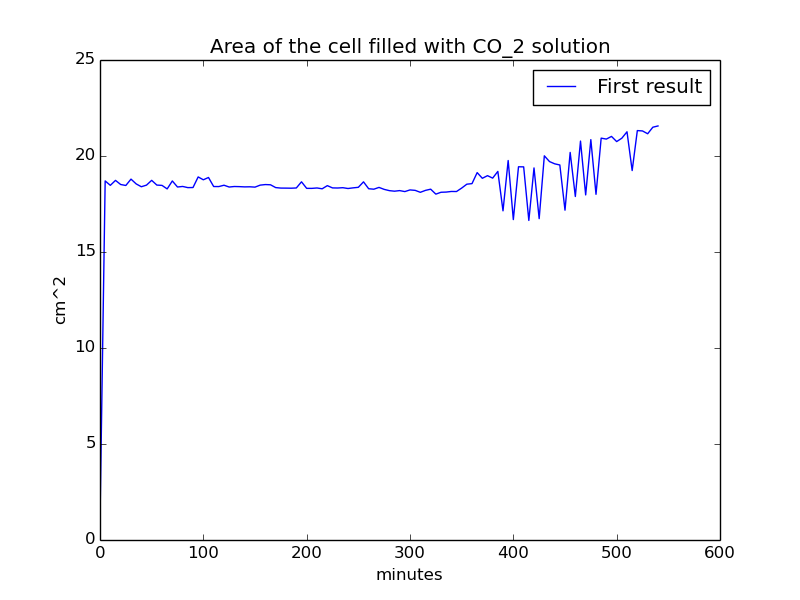
\includegraphics[width=0.55\textwidth]{area_1.png}\label{fig:area1_bad}
\captionof{figure}{Plot of the area with our second plate}
\vspace{0.3cm}
We had to adjust the ImageJ quite a bit to fit the above graph properly and this is the best we could come up with, we shall mention why it is the way it is in the next section. 
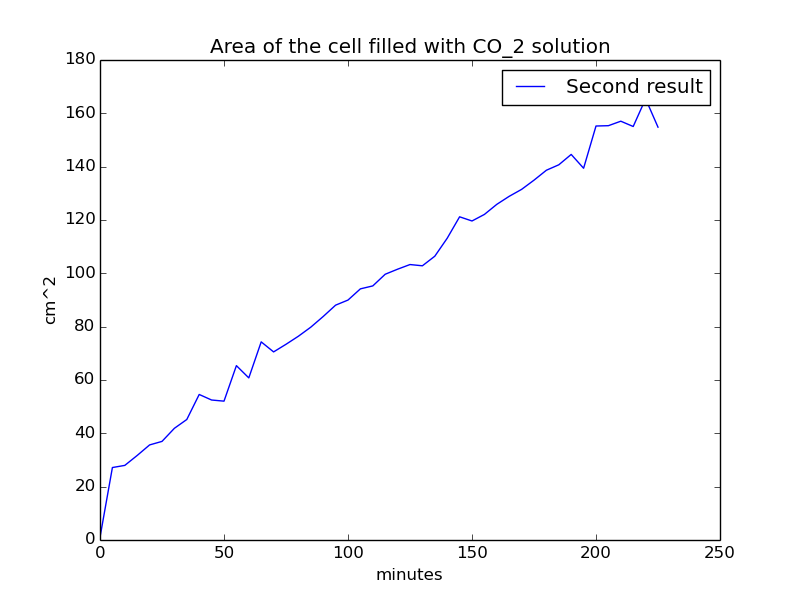
\includegraphics[width=0.55\textwidth]{area_2.png}\label{fig:area3_45}
\captionof{figure}{plot of our second clear result} 
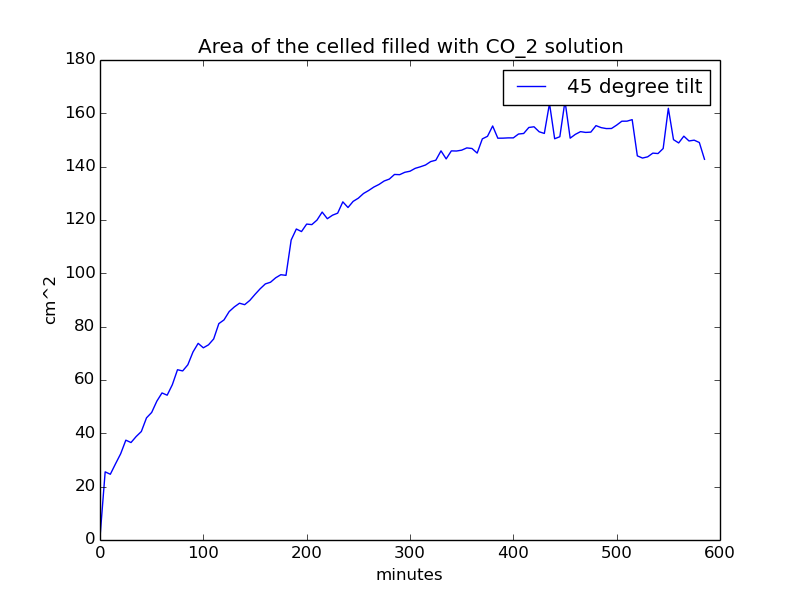
\includegraphics[width=0.55\textwidth]{area_3.png}\label{fig:area2_good}
\captionof{figure}{Plot of the area with the second plate with 45 degrees tilting} 
\vspace{0.1cm}
We also had once successful tilting which gave result at $45$ degrees as seen in the following Figure 20. The area with no tilting involved is shown in Figure 21.
We tried lowering the system even lower to around $14$ degrees, with no successful results\\

\includegraphics[width=0.50\textwidth]{DSC_3327.JPG}\label{fig:14d}
\captionof{figure}{At 14 Degrees} 

%------------------------------------------------
\newpage
\section{Discussion}
As we can see from the photos and graphs from the previous sections we have stumbled upon quite a few problems. 
\subsection{Initial plate}
When it comes to our initial plate we clearly see from the photos that it was a total failure. There are varied reasons for this referring to figure ~\ref{fig:first_attempt} we see that we had our solution way above the level of beads and not enough room for the CO$_2$ to slowly spread and dissolve. Furthermore we used 1mm beads in a gap $0.9$cm this made it really hard for the density driven convection to appear and thus our 2D model failed. \\
On the figure ~\ref{fig:second_attempt} we see that by using bigger sized beads does help a little but this poses another problem in that way that we see crystal formations taking place and thus making it very hard to distinguish the fingers from the rest if we look closely on the figure mentioned we can see what looks like a finger but because of the pattern formed by the beads it is hard to distinguish it. Perhaps if there was a bigger contrast between the fingers and the solution we might have been able to see it slightly better. \\
On our third trial, referring to figure~\ref{fig:third_attempt} by mixing it solved the problem of crystal patterns appearing, but it did not solve the problem of keeping the system in 2D and by that we mean there were too many beads inside a small volume not giving the fingers the ideal environment to form and the BTB solution is very dark making bad conditions for the light to pass through the thick glass and beads to reach the camera.\\ 
In our last experiment with this system, the system failed as there was no CO$_2$ injection taking place and we see that the solution has dried up leaving the upper beads in contact with open air. 

\subsection{Second plate}
After the fourth try and seeing no valid results we decided to switch to a thinner and glass plate with a gap size $0.5$cm. We got the idea of switching once we got to know that the group from last year used a gap equivalent to the tube diameter (ours was narrower than that as we had to squeeze the tube in). Using the new set up and pitch perfecting our solution concentration and choosing a constant beads size to experiment with we finally got some results worth analysing. From figure~\ref{fig:timevo} we finally get to see that as the density driven convection takes place the number of fingers keeps increasing and thus also the area it covers. We would expect to see a linear function plotting the area against time and this can clearly be seen in figure~\ref{fig:area2_good} as we would expect. \\
Once we tilt it around $45$ degrees we see that we still get a relatively linear curve. It remains to be seen how much lower one can tilt the system before the fingers stop showing up, as we have shown on figure~\ref{fig:14d}. We one at $21$ degrees as well which had failed similarly.\\ 
We also note that as the fingers are forming they propagate vertically and horizontally at a steady velocity. The fingers interact and merge with each other until eventually the process stops as the fingers get closer to the edges and get mixed with the solution.
\subsection{Conclusion} % (fold)
\label{sub:conclusion}
In our experiments we have had many errors and miscalculation, among them when mixing the BTB solution we were not measuring with significant accuracy, the angles we measured were just approximations and subject to around $\pm 2$ degrees, but these numbers should not play a significant role in the bigger part of the experiment which is to see whether the patterns show up and study them. We had the experiments done on several angles 45,14 and 21 degrees, but as can be seen from the plot only the 45 degree experiment gave any measureable result the rest were just failures. One of the bigger problems was to get the software ImageJ to work as there was limited documentation concerning our type of project, thus making us rely on trial and error which occupied much of our time. Another huge fallback was the lack of a proper report from those who have done this experiment last year, thereby making us once again go through all the basic procedures all over again such as BTB mixing and experimental set up. Concerning our results and last years, we cannot really make any comparison concerning the data but concerning the set up, we had a far higher stability when it comes to our system. \\
Last year's group had the tube between the two plates which they tightened with clamps. We had to use their set up and this was not a wise set up as the cleaning process was more difficult than ours since in this case we had to remove the above plate and then the tube while slowly swiping the beads away. Ours was by no means perfect as we stumbled upon the problem of pouring in the beads into the narrow gap, now in our initial plate this was not an issue but the issue became significant once we went over to the smaller gap sized glass plates, specially when the beads were wet then it would get harder to fit in the beads and fill up the glass plate. In the future possibly things to consider investigating is the tilting and at which angle the fingers stop forming and if one has the time one could also calculate the velocity of the fingers compared to the width to see the relation between them. 
% subsection conclusion (end)
%----------------------------------------------------------------------------------------
%	REFERENCE LIST
%----------------------------------------------------------------------------------------
\end{multicols}
\newpage
\begin{thebibliography}{99} % Bibliography - this is intentionally simple in this template

\bibitem{Figure1}
Figure~\ref{fig:ccs}\\
\url{http://www.altenergymag.com/emagazine/2013/04/overview-of-carbon-capture/2068}

\bibitem{groundwater}
Weir et al.,
1996; Lindeberg and Wessel-Berg, 1997; Ennis-King et al.,
2005; Riaz et al., 2006; Hidalgo and Carrera, 2009; Pau
et al., 2010; Kneafsey and Pruess, 2010; Neufeld et al.,
2010].

\bibitem{Hassan07}
Hassanzadeh, H., Pooladi-Darvish, M. and Keith, D.
(2007). Scaling behavior of convective mixing, with
application to geological storage of CO2. AIChE journal,
53(5), pp.1121--1131.

\bibitem{BTB}
Gabriela Braganca Costa e Moreira and Bjornar Sandnes[Role of Bromothymol Blue pH Indicator in Density
Driven Convection of Carbon Dioxide Saturated
Water]

\bibitem{pump}
Figure~\ref{fig:pump}\\
\url{http://www.southpointesurgical.com/images%5Cne1600.jpg}

\bibitem{imagej}
\url{http://fiji.sc/Fiji}
\end{thebibliography}

%----------------------------------------------------------------------------------------



\end{document}